\documentclass[a4paper,twocolumn]{article}
\usepackage[utf8]{inputenc}
\usepackage[T1]{fontenc}
\usepackage{amsmath}
\usepackage{graphicx}
\usepackage{listings}
\usepackage[english]{babel}
\usepackage{xcolor}
\usepackage{subcaption}
\usepackage[capitalise]{cleveref}
\usepackage{fancyvrb}
\VerbatimFootnotes

\usepackage[ddmmyy]{datetime}

\title{Making Publication Quality Figures}
\author{Sigvald Marholm}
\date{\today}

\newcommand{\dd}{\mathrm{d}}
\newcommand{\half}{\frac{1}{2}}
\newcommand{\n}[1]{\bar{#1}}
\newcommand{\nd}[1]{\tilde{#1}}
\newcommand{\refeq}[1]{(\ref{eq:#1})}
\newcommand{\reffig}[1]{Fig.~\ref{fig:#1}}
\newcommand{\reftab}[1]{Tab.~\ref{tab:#1}}
\newcommand{\refli}[1]{Listing~\ref{li:#1}}
\newcommand{\const}{\mathrm{const}}
\newcommand{\cd}{\texttt}
\renewcommand{\vec}{\mathbf}
\renewcommand{\dateseparator}{.}

\makeatletter
\newcommand{\extract}{
\noindent
Text width: \the\textwidth.\\
Column width: \the\columnwidth.\\
Line width \the\linewidth.\\
Font family: \f@family.\\
Text size: \f@size pt.
}
\makeatother

\makeatletter
\newcommand{\getfont}{\f@family~\f@size pt}
\makeatother

\begin{document}

\maketitle
\pagebreak

% \setcounter{section}{-1}
\section{Introduction}
It is not uncommon to see technical reports and scientific articles with figures of different style than the rest of the document.
The text in the figures may be too small or too large, the wrong font may be used, the lines in plots so thin they are barely visible, or figures may appear pixelated when printed due to insufficient resolution.
\Cref{fig:poorfig} is an example of such a figure.
Although it is quite understandable that such figures appear, there is a very simple recipe for avoiding them\footnote{Admittedly, there are other ways too, for instance making figures directly in \LaTeX{} using PGF or Tikz, but this recipe has become my preferred way. Note that vector graphics is not a replacement for the recipe. It gives you an easy way out when it comes to resolution, but text sizes and line widths gets scaled unless care is taken.}:
\begin{enumerate}
    \item Obtain the correct figure size and font from the document where the figure is to be inserted.
    \item Create the figure using the right sizes, font and resolution from the start. For consistency between figures you may use the same line width, color palettes, etc. in all your figures.
    \item Import the image into the document \emph{without} rescaling it.
\end{enumerate}
The only difference between \cref{fig:poorfig} and \cref{fig:goodfig} is that the latter was made according to the above recipe.

\begin{figure}
    \begin{subfigure}{\linewidth}
        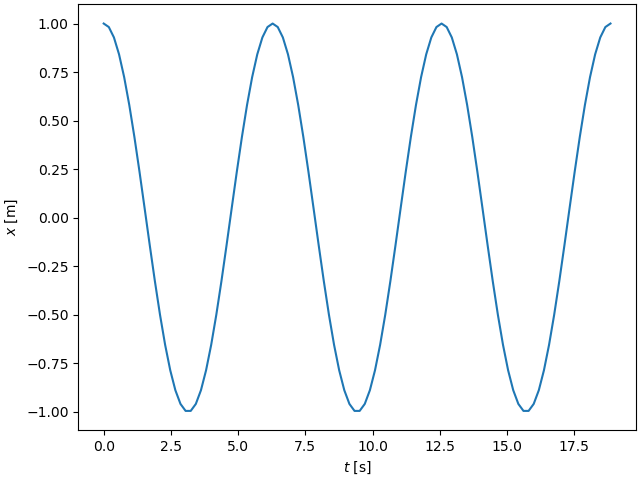
\includegraphics[width=\columnwidth]{poorfig.png}
        \caption{Poor figure}
        \label{fig:poorfig}
    \end{subfigure}
    ~\\

    \begin{subfigure}{\linewidth}
        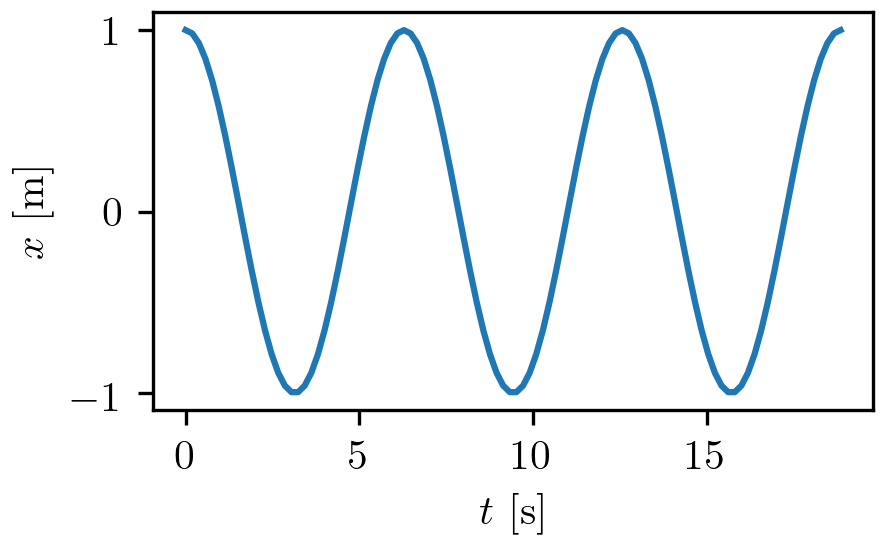
\includegraphics{goodfig.png}
        \caption{Good figure}
        \label{fig:goodfig}
    \end{subfigure}
    \caption{Example figures}
\end{figure}

In this document I shall explain how to carry out the above steps in practice, as well as some tricks for an efficient workflow.
This being about publication quality, I assume \LaTeX{} is used for typesetting, but demonstrate how to best incorporate figures from a selection of high quality graphics tools such as Matplotlib and Inkscape.
That said, this is not an exhaustive tutorial on those tools, or on the artistic aspects of figure making.

% The reader familiar with vector graphics should note that vector graphics is no replacement for the above recipe.
% Although vector graphics can be scaled to fit inside any document without loss of quality, this scaling also affects the text such that it quickly becomes too small or too large.
% You would also not get consistent line widths, arrow sizes, etc., between your figures should you attempt that, because they may be scaled by different factors in different figures.

% In what follows, we go through each step in detail.
% In step 2 there is obviously endless possibilities in which software to use, and how to use them, and we do not cover it all.
% We do, however, provide some general information, as well as some relevant details on getting the right figure size in a few selected tools: InkScape, Gimp, and Matplotlib.

\vfill

\section{The Recipe}

\subsection{Step 1: Extract font and sizes}

\subsubsection{Figure Size}
We shall start by determining the right size of the figure.
For two-column articles one may for instance let the figure fill the entire column width, whereas for single column articles perhaps a lower fraction of the width is more suitable.
In any case, it is a good start to know what the column width \emph{is}.

The column width is not the same on all documents, but fortunately, it is rather easy to extract by inserting the following \LaTeX{} command somewhere in your document:
\begin{verbatim}
\the\columnwidth
\end{verbatim}
When the document is compiled, the width of the column will be written in place of this command, for instance ``221.0pt'' for a typical two-column document. 
In case you have a very wide figure and would like it to span both columns (using the \verb|figure*| environment), you should instead insert
\begin{verbatim}
\the\textwidth
\end{verbatim}
The text width accounts for both columns, as well as the spacing in between.
For single column documents the text width and the column width are usually the same.

Although many programs allow you to specify the size of a figure directly in typographic points (pt), one should be aware that slightly different definitions of the pt exists.
This usually isn't noticable when specifying the text size, which is usually around 10pt.
However, if a figure ends up slightly wider than a column, you will get an ``overfull hbox'' warning by \LaTeX{}.
You may therefore wish to convert the column width to for instance millimeters or inches before creating the figure.
In \LaTeX{}, the conversion is given by
\begin{align}
    1\,\mathrm{pt} = 0.351\,\mathrm{mm} = 0.0138\,\mathrm{in}.
\end{align}
A column width of for instance $221\,\mathrm{pt}$ thus converts to $77.6\,\mathrm{mm}$.
If you want a full width figure, it pays off to round downwards, for instance to $77\,\mathrm{mm}$, to make sure you don't get an ``overfull hbox''.
The height of the figure is simply chosen to get an aspect ratio deemed appropriate for the figure. I sometimes take the width multiplied or divided by 1.618 to get the golden ratio.

% \subsubsection{Extract}
% \extract

\subsubsection{Font and Text Size}
The next thing we need is to determine the font family and text size. This can be found by inserting the following into your document\footnote{
The macro \verb|\f@family| contains the font name and the macro \verb|\f@size| the text size. The \verb|@| symbol is frequently used in macro names internal to \LaTeX{} packages to prevent them from being overwritten by the end user.
The reason this works is because \verb|@| behaves as a normal letter inside packages and that it can therefore be used in macro names.
During normal usage, however, \verb|@| is a special symbol.
Nevertheless, we can temporarily turn \verb|@| into a normal letter with \verb|\makeatletter| to get access to these macros, and then turn it back to a symbol again using \verb|\makeatother|.
This is what we have done in the above code.
}:
\begin{verbatim}
\makeatletter
\f@family~\f@size pt
\makeatother
\end{verbatim}
To make it a bit more convenient, the following code can be put in the preamble of your document:
\begin{verbatim}
\makeatletter
\newcommand{\getfont}{\f@family~\f@size pt}
\makeatother
\end{verbatim}
Now you can just insert \verb|\getfont| where you want to determine the font. Note that the text size often differs in foonotes, figure captions and in the body of the document.
A good result can be obtained by using a text size in the figures that is identical to that in the figure caption. You may of course choose differently, as long as you do it consistently.
% You should also be aware that the text size (or sometimes even the font) may be different on different parts of your document. The footnotes, for instance, are typically smaller. The figure captions are also sometimes a bit smaller than the body text. If that is the case, it would make sense for the text inside your figures to match the size of the figure captions rather than the body text. You may also deliberately choose a slightly smaller text size inside your figures as part of your document's style, e.g. 9pt instead of 11pt. This is fine as long as you do it consistently throughout your document.

The output from the above command may be something like ``cmr~10pt''. cmr is short for Computer Modern Roman, which is the standard font in \LaTeX{}.
% The font families in \LaTeX{} often do not come out with nice names such as ``Times New Roman'' but may instead come out as something like ``cmr''. ``cmr'' is short for Computer Modern, the standard font in \LaTeX{}.
Unfortunately the font format used in \LaTeX{} is a different kind than the TrueType or OpenType formats understood by most programs, and it may therefore be difficult to find the exact same font for use in your graphics software. Computer Modern, however, often have good replica available for download on the internet. If you are unable to find the exact same font, you may instead use something similar. Computer Modern or variants of Times or Times New Roman are often used fonts in scientific journals.

One thing in particular to pay attention to is whether or not the fonts have \emph{serifs}, i.e., tiny feet on letters such as ``i'' and ``f'':
\\
~

{ \hfill {\Huge Serif} \hfill {\Huge \sf Sans Serif} \hfill }
\\

\noindent Fonts may be classified into serif fonts or sans (without) serif fonts according to this feature.
It is interesting that the serifs almost touches one another at the base of each line, thereby creating the illusion of a continuous line on which the letters sit.
There is also the illusion of a line on top of the ``low'' letters.
These lines are believed to help guide the eye along the text, preventing you from losing track of which line you're currently reading.
Serif fonts are therefore the norm when it comes to printed books and articles, perhaps except for headings, or where there are only small fragments of text.
Sans serif fonts, on the other hand, can be used with lower resolution, and are predominant on web pages, and other digital resources. Plotting tools such as Matplotlib often uses a sans serif font by default. Choosing \emph{any} serif font in your plots goes a long way for a more consistent look. Compare for instance \cref{fig:poorfig} to \cref{fig:goodfig}. The former uses the default sans serif font in Matplotlib, whereas the latter uses Computer Modern, which is also used in the rest of this document.

\subsection{Step 2: Create the Figure}
Regardless of what software you use for creating your figures, you ought to use a suitable image format, and choose an appropriate resolution. If you fail at this, the picture may be grainy or show compression artefacts on print, or the file size of the document may become very large. Many journals have rather strict size limits on the submitted files. In this section I elaborate on which file formats to use and resolution requirements while postponing details about specific software for making images until later.

% Let us first discuss what is common regardless of what software you choose for creating your figures.
% First you need to choose a suitable image format with respect to both quality and size. Some journals have a file size limit on the submitted documents, but if you habitually use the correct format ind image size this should not pose any problem. We present a summary of formats below:

\subsubsection{Image Formats}
\begin{description}
    \item[BMP] This is one of the simplest formats, where an image is represented as a grid of pixels (a \emph{raster}) with each pixel stored as a fixed number of bytes. This leads to comparatively large files. Use PNG or JPG instead.
    \item[PNG] Similarly to BMP, this is also a raster format, but contrary to BMP, it uses a \emph{lossless} compression scheme, meaning that it takes less space with no loss of quality. Save the files with compression level 9 to get the smallest files. The compression used in PNG is efficient for images where large areas have the same color, typically graphical illustrations, schematics and plots. The compression is not as efficient for photographs, although it does lead to significantly smaller files than BMP.
    \item[JPG] Yet another raster format, but this one with a \emph{lossy} compression, leading to a quality reduction. For JPG you can tune a quality factor between 0 and 100, where a higher number means better quality, but larger files. JPG files are very well suited for photographs, and even a quality factor of 90 or 95 will produce files much smaller than PNG files at still an excellent quality. The JPG compression do not handle sharp edges very well, where ``foggy'' artifacts may become visible, especially for lower quality factors. This makes it in particular unsuitable for graphical illustrations, schematics and plots, where there are large single-color regions with sharp edges between.
    \item[SVG] Contrary to the previous formats, SVG is a \emph{vector} format, meaning that it consits of geometric entities such as lines and curves being described by their end points, curvature, thickness, etc. Whereas the pixels would become visible if you scale up a raster format, the vector formats can be scaled up indefinitely without getting pixelated. For this reason, vector graphics is excellent for graphical illustrations and schematics, but the figures must be created using a dedicated program, such as InkScape, from the very start. You cannot convert a raster image into a vector format. Although it is sometimes possible to store plots in vector formats, this means storing every single line segment in the plot, which can potentially be quite many, and this causes needlessly large files. For that reason I have come to prefer PNG files for plots of real data. Unfortunately, \LaTeX{} cannot import SVG files, so they must be converted to PDF files prior to being used in \LaTeX{}. However, SVG files is the native format for many programs, and keeping a copy of the figure also in SVG enables you to more simply make adjustments later on.
    \item[PDF] In addition to full fledged documents, PDF files can also be used to store vector graphics, as described above.
    \item[EPS] If you compile your documents using the command \verb|latex|, none of the above formats can be used, and you must instead resort to EPS. EPS can also store raster and vector graphics, but I recommend rather compiling your documents with the more modern \verb|pdflatex| if possible.
\end{description}

Although vector formats can be scaled without loss of quality, it is still desirable to create figures with the right dimensions to begin with, as determined in step 1. This means that if you insert text with a size of, say, 10pt in your graphics program, it will appear as 10pt in \LaTeX{} because you do not have to scale the figure. You can also standardize dimensions such as line thicknesses and arrow sizes to your liking to get a consistent look throughout your entire document.
When using raster formats, it is in addition necessary to have a sufficiently good resolution.

\subsubsection{Resolution}
The resolution of your monitor can be measured in \emph{pixels per inch} (PPI). If, for instance, you have a 14 inch laptop monitor with $1920\times1080$ pixels\footnote{The number of pixels per dimension is also usually referred to as resolution, but that is actually a misnomer, since it does not say anything about how dense the pixels are.}, there will be
\begin{align}
    \sqrt{1920^2+1080^2}=2202.9
\end{align}
pixel lengths along the diagonal, and hence your monitor has a resolution of
\begin{align}
    2202.9 / 14 = 157
\end{align}
pixels per inch. Larger screens often have the same number of pixels, and thus a lower resolution. If you display a $300\times300$ pixel image on full scale on this monitor, the image would be $300/157=1.91$ in each side, or 4.85 cm, using the conversion 
\begin{align}
    1\,\text{in} = 2.54\,\text{cm}.
\end{align}

The resolution on print works similarly, except that it is usually referred to as \emph{dots per inch} (DPI), and that it must be specified in the image file (or file to be printed). For an image to appear of good quality on print, a resolution of 300 DPI is advisable. With this resolution, the $300\times300$ pixel image would be only one inch, or 2.54 cm each side. Higher resolution leads to larger files, whereas lower resolution may result in a seemingly good quality on screen, but not necessarily when printed. With this knowledge, a single column figure of 77 mm width would require a width of $300\cdot7.7/2.54=909$ pixels to look good on print. Fortunately, it is usually possible to specify size and resolution separately in graphics editors, such that you would only have to specify 77 mm, whatever height you find suitable and 300 DPI. Text is inserted with whichever font and text size previously determined.

\subsection{Step 3: Inserting the Figure}
Finally comes the point of inserting the figure into your \LaTeX{} document.
If everything went according to the plan, it should be enough to write

\begin{verbatim}
\includegraphics{file.png}
\end{verbatim}
(given that the file is named \verb|file.png|). Note that we do not use any options for scaling the figure, like \verb|[scale=0.23]| or \verb|[width=0.7\columnwidth]|. The default is already a scaling factor of one, which means that the figure would appear on print with 300 DPI and a width of 77 mm for the example used throughout. If, for some reason, you were not able to set the DPI correctly, the figure will out-of-scale. As a last resort you can then specify the size manually, e.g.,
\begin{verbatim}
\includegraphics[width=77mm]{file.png}
\end{verbatim}
and if the image has the correct number of pixels, it will still be 300 DPI when it is actually printed.

\subsection{InkScape}
\subsection{Gimp}
\subsection{Matplotlib}
\subsection{ImageMagick}


That's all, good luck!
\end{document}
